\documentclass{beamer}
\usepackage{verbatim}
\usepackage{graphicx}
%% \usetheme{}
%% \usecolortheme{}
%% \usefonttheme{}
\title{Benchmarking Parsers}
\author{Nikolaos Bezirgiannis}
\date{\today}
\begin{document}

%% Title
\begin{frame}
\titlepage
\end{frame}

%% TOC
\begin{frame}{Outline}
\begin{itemize}
\item Intro
\item Parser Combinator Libraries
\item Benchmark Results
\item Outro
\end{itemize}
\end{frame}

\section{Intro}

\begin{frame}{State of Parsing}
\begin{itemize}
\item Parser Generators
  \pause
  \begin{itemize}
    \item Yacc / Bison
      \begin{itemize}
        \item LALR(1) algorithm
        \item Accompanied by a lexer (e.g. lex / flex)
        \item Generates code for C / C++ / Java
      \end{itemize}
      \pause
    \item ANTLR
      \begin{itemize}
        \item LL(*) algorithm
        \item Generates code for many languages
        \item GUI tools: editor, interpreter, debugger, visualization utilities
      \end{itemize}
      \pause
    \item Happy
      \begin{itemize}
        \item Written in Haskell
        \item Generates Haskell
        \item Accompanied by Alex (also in Haskell)
        \item Pretty solid \& stable
      \end{itemize}
  \end{itemize}
  \pause
\item Parser Combinators
\end{itemize}
\end{frame}

\begin{frame}{Combinatory Parsing}
  \begin{itemize}
  \item A \textbf{parser} is a function that consumes input and returns some structure.
  \item A \textbf{parser combinator} is a higher-order function that takes parsers to form a new larger parser.
  \item The \textbf{parsing program} is the application of some basic parsers and parsing combinators.
  \end{itemize}
\end{frame}

\begin{frame}{Combinatory Parsing (cont.)}
  \begin{itemize}
  \item Advantages
    \begin{itemize}
    \item Readable
    \item Written in the same programming language
    \item Can be extended by the user with new parsers and combinators
    \item Maintainable
    \end{itemize}
  \item Disadvantages
    \begin{itemize}
    \item No grammar analysis
    \item No left-recursion 
    \item Some cases have high time and space usage
    \end{itemize}
  \end{itemize}
\end{frame}

\begin{frame}{History of Combinatory Parsing}
  \begin{itemize}
  \item Wadler, 85: \emph{List of Successes} method
  \item Wadler, 92: Monadic Parsers
  \item Hutton, 92: basic parser combinators (in Miranda)
  \item R\"ojemo, 95: Applicative Parsers
  \item Hutton,Meijer, 96: Standardizing parser combinators, a Hugs parsing library
  \item Leijen,Meijer, 01: Parsec, fast parsing library with good error reporting
  \item Swierstra, 01: Applicative parsers with error correction
  \item Swierstra, 04: Permutation parsing
  \item Swierstra, 06: Online results parsing
  \end{itemize}
\end{frame}

\section{Parser Combinator Libraries}

%% Maybe short them by date

\subsection{parsec}

\begin{frame}{Parsec2}
\begin{itemize}
\item Written by Daan Leijen
\item Introduced in 2001
\item Became de-facto
\item Used to be distributed with GHC
\item Now distributed with Haskell Platform
\end{itemize}
\end{frame}

\begin{frame}{Parsec2 Features}
\begin{itemize}
\item Parses context-sensitive grammars
\item Predictive LL(1) by default
\item LL(*) by explicit backtracking
\item Monadic Interface
\item Permutation parsing
\item Good error messages (Position, Unexpected Input, Expected production)
\item Haskell98-compatible
\end{itemize}
\end{frame}

\begin{frame}{Parsec2 Drawbacks}
\begin{itemize}
\item Lacks an applicative interface
\item Accepts a token-list as input
\item Cannot be used with Bytestring or Text
\end{itemize}
\end{frame}

\begin{frame}{Parsec3}
\begin{itemize}
\item In most cases, API-compatible to Parsec2
\item Adds an applicative interface
\item Parameterized over the input type
\item Provides the parser as a monad transformer
\item Breaks Haskell98-compatibility
\item Trying to be flexible, it pays in terms of speed
\end{itemize}
\end{frame}

\subsection{uulib}

\begin{frame}{UUlib General}
\begin{itemize}
\item Written by UU
\item Introduced $<$ 2005
\item Stable
\item The library bundles also a lexer and a prettyprinter
\end{itemize}
\end{frame}

\begin{frame}{UUlib Features}
\begin{itemize}
\item Applicative Interface
\item Good Error reporting
\end{itemize}
\end{frame}

\begin{frame}{UUlib Drawbacks}
\begin{itemize}
\item Lacks a monadic interface $\Rightarrow$ difficult to construct context-sensitive grammars
\item Does not have pSatisfy.It makes difficult to construct some basic parsers.
\item Not documented
\item Restricted only to String input
\end{itemize}
\end{frame}

\subsection{uu-parsinglib}

\begin{frame}{UU-parsinglib General}
\begin{itemize}
\item Written by Doaitse Swierstra
\item Introduced in 2008
\item Somewhat stable
\end{itemize}
\end{frame}

\begin{frame}[fragile]{UU-parsinglib Features}
\begin{itemize}
\item LL(*)
\item Applicative and Monadic Interface
\item API-compatible with uulib
\item Good at dealing with ambiguity
  \begin{itemize}
    \item Guesses out when the grammar is ambiguous and reports it
    \item \verb|amb :: Parser a -> Parser [a]|
  \end{itemize}
\item Compared to the other libraries, it seems to be the best abstracted away
\item Great Error messages
\item Error Correction
\item Online parsing results
\item Visits the alternatives in parallel (BFS), so it does not retain the whole input in memory
\item Input can also be Bytestring,Text,etc
\item Extremely easy to switch between input types (thanks to ListLike)
\end{itemize}
\end{frame}

\begin{frame}{UU-parsinglib Drawbacks}
\begin{itemize}
\item Error Correction cannot be used with the monadic interface
\item Underdocumented
\item The abstractions make it harder for beginners to understand the lib
\end{itemize}
\end{frame}

\subsection{attoparsec}

\begin{frame}{Attoparsec General}
\begin{itemize}
\item Written by Bryan O'Sullivan
\item Introduced in 2007
\item Has recently become very popular
\item Starting to mature
\end{itemize}
\end{frame}

\begin{frame}{Attoparsec Features}
\begin{itemize}
\item LL(*) , implicit backtracking
\item Applicative and Monadic Interface
\item Supports Text, Bytestring
\item Supports Incremental Input % this can be done in Parsec and other libraries with Lazy IO, but this is better
\item Nearly translatable/compatible with Parsec
\item Easy to use, by having distinct modules
\end{itemize}
\end{frame}

\begin{frame}{Attoparsec Drawbacks}
\begin{itemize}
\item Trying to stay simple, it lacks some high-level combinators
\item Not good in error reporting
\item Does not accepts String input 
\end{itemize}
\end{frame}

\subsection{polyparse}

\begin{frame}{Polyparse General}
\begin{itemize}
\item Written by Malcolm Wallace
\item Introduced in 2002
\item Is actually a collection of different parsing libraries
\end{itemize}
\end{frame}

\begin{frame}{Polyparse Features}
\begin{itemize}
\item LL(*) with implicit backtracking
\item Applicative and Monadic Interface
\item Partial parsing results 
\item Supports String, ByteString and Text for input
\end{itemize}
\end{frame}

\begin{frame}{Polyparse Drawbacks}
\begin{itemize}
\item The library's schema is confusing
\item Lacks some high-level combinators for Text
\end{itemize}
\end{frame}

\section{Results}

\begin{frame}[fragile]{CSV - Example}
\begin{itemize}
\item Comma-separated values
\item Has a standard but many variations exist
\item Our parsers support the standard with unicode
\item Datasets taken from the net
\end{itemize}
\begin{verbatim}
dma code,region,state
500,Portland-Auburn,ME
501,New York,NY
502,Binghamton,NY
503,Macon,GA
504,Philadelphia,PA
505,Detroit,MI
506,Boston,MA
507,Savannah,GA
508,Pittsburgh,PA
\end{verbatim}
\end{frame}

\begin{frame}{CSV - Time}
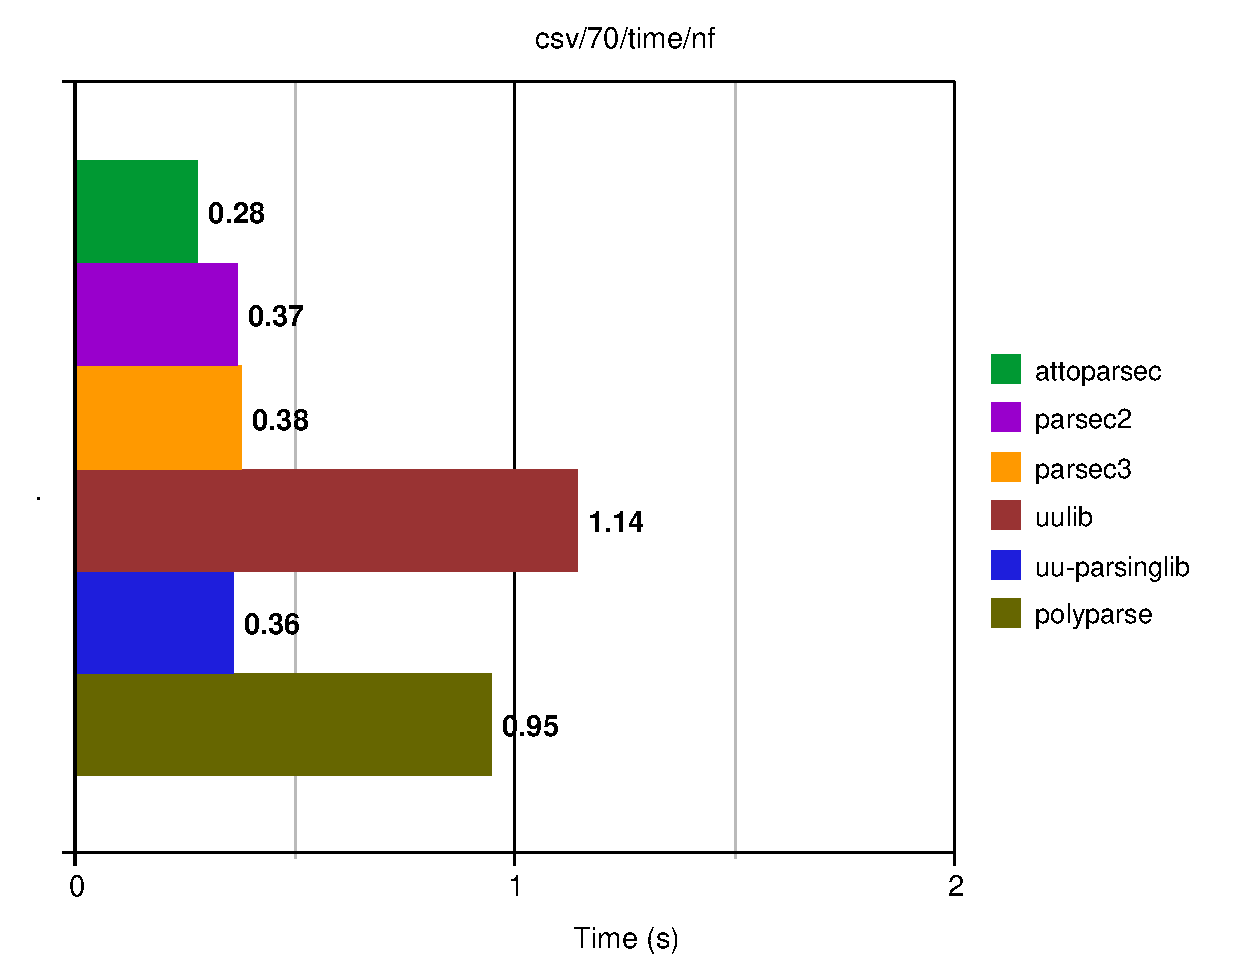
\includegraphics[scale=0.5]{presentation/csv-70-time-nf.pdf}
\end{frame}

\begin{frame}{CSV - Time - 74}
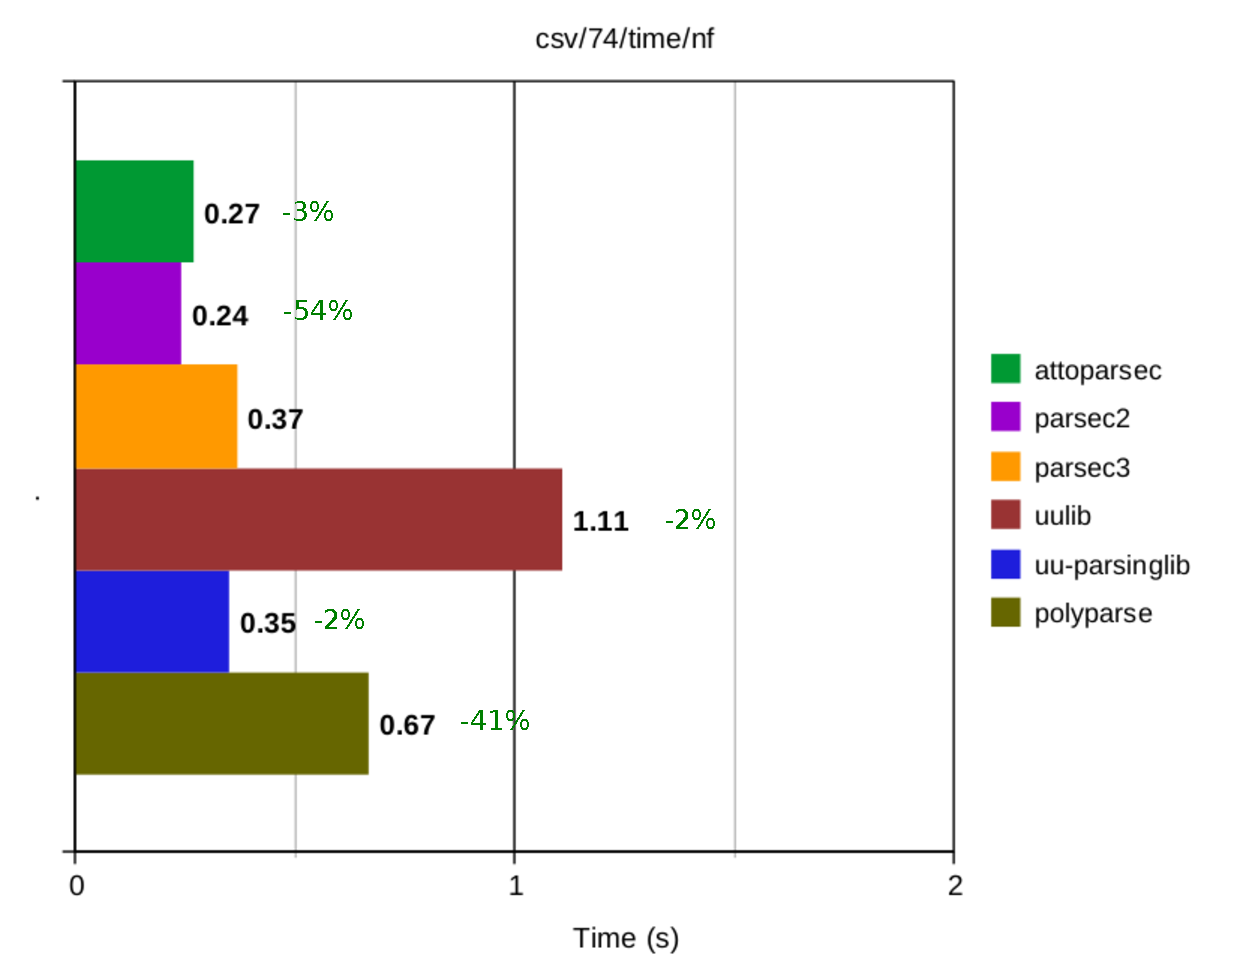
\includegraphics[scale=0.5]{presentation/csv-74-time-nf_.pdf}
\end{frame}

\begin{frame}{CSV - Space}
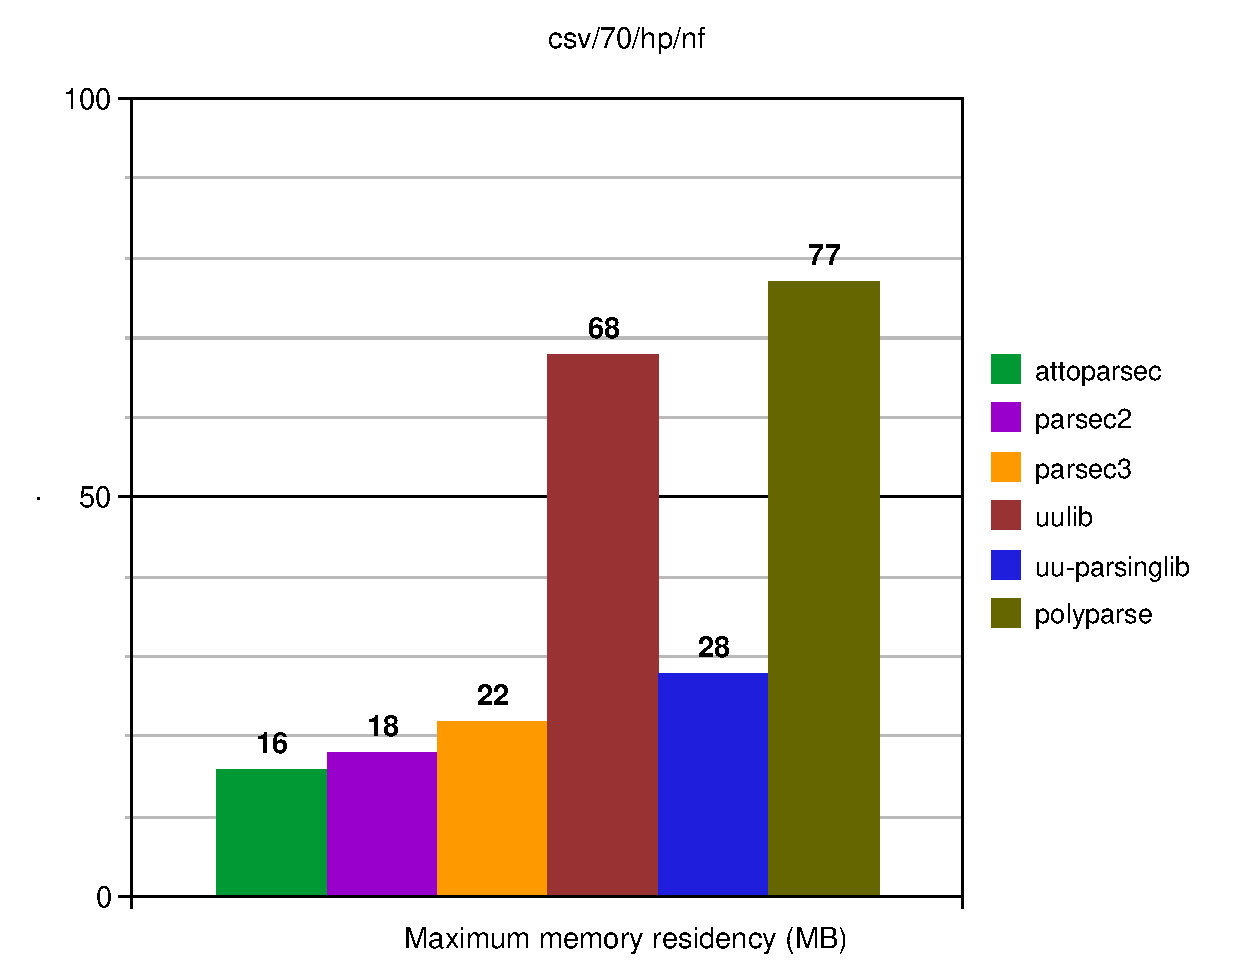
\includegraphics[scale=0.5]{presentation/csv-70-hp-nf.pdf}
\end{frame}

\begin{frame}[fragile]{EXPR - Example}
\begin{itemize}
\item a small custom functional language
\item Datasets generated with QuickCheck's Arbitrary
\end{itemize}
\begin{verbatim}
((2 - let nngxpu = (kpjht + (lms + (medpc - l))) in 
(let sk = yui in o + ((qatzrb * 2) - (8 - 2)))) - 
(((let idwxvj = let ywkldp = 5 in c in (5 * az) 
* (8 * let rh = yo in h)) + (((awpcu - 2) - (tcwhem * 
nyt)) * let pm = (5 * lttgyt) in (cl + 5))) - 
((((bf - 3) * (7 * 7)) - ((7 * vpienh) + (dy + 6))) 
+ (((8 + 6) - (7 * 7)) + let zvs = poks in (2 * sfwo)))))
\end{verbatim}
\end{frame}

\begin{frame}{EXPR - Time}
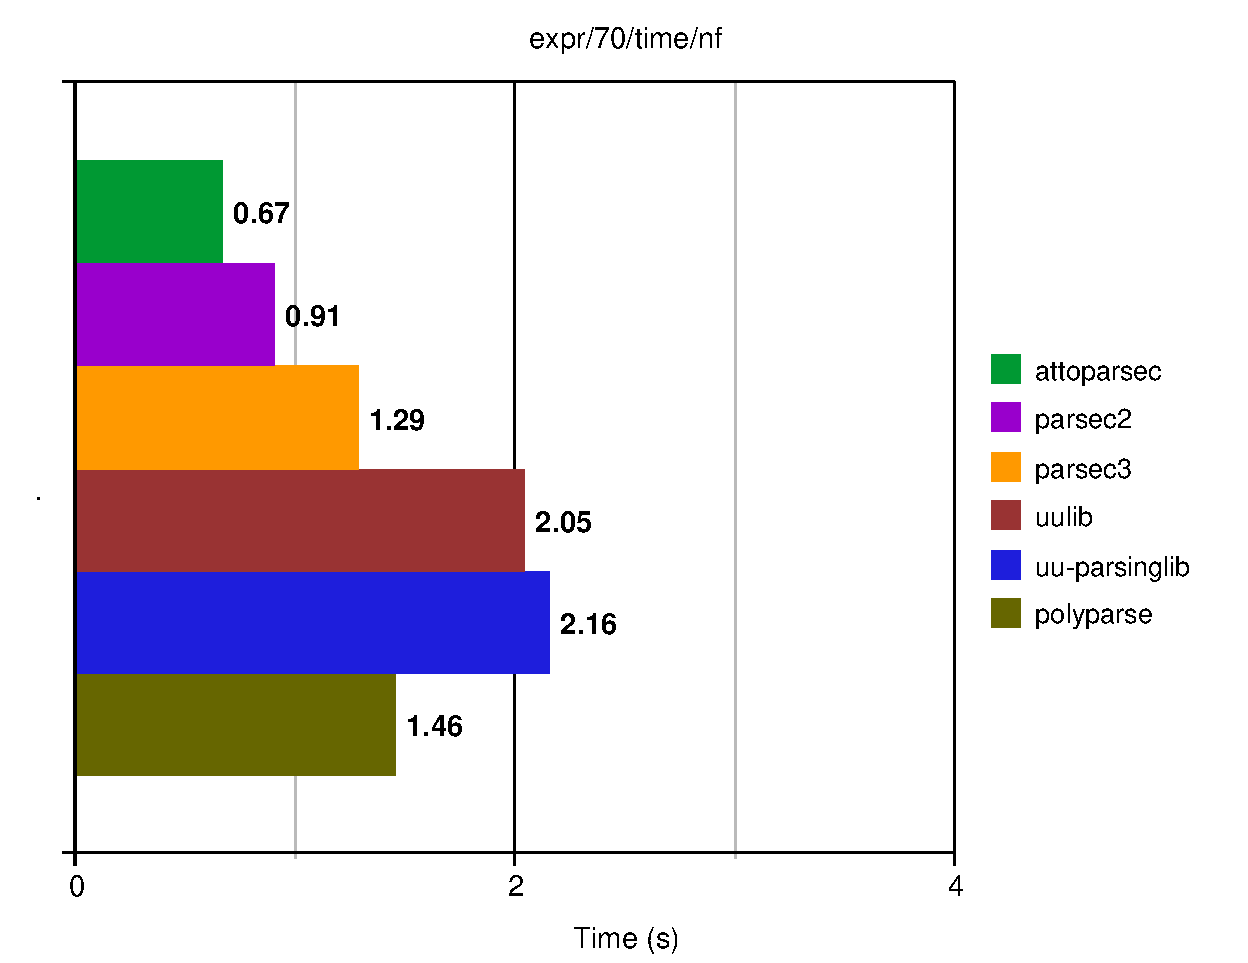
\includegraphics[scale=0.5]{presentation/expr-70-time-nf.pdf}
\end{frame}

\begin{frame}{EXPR - Time - 74}
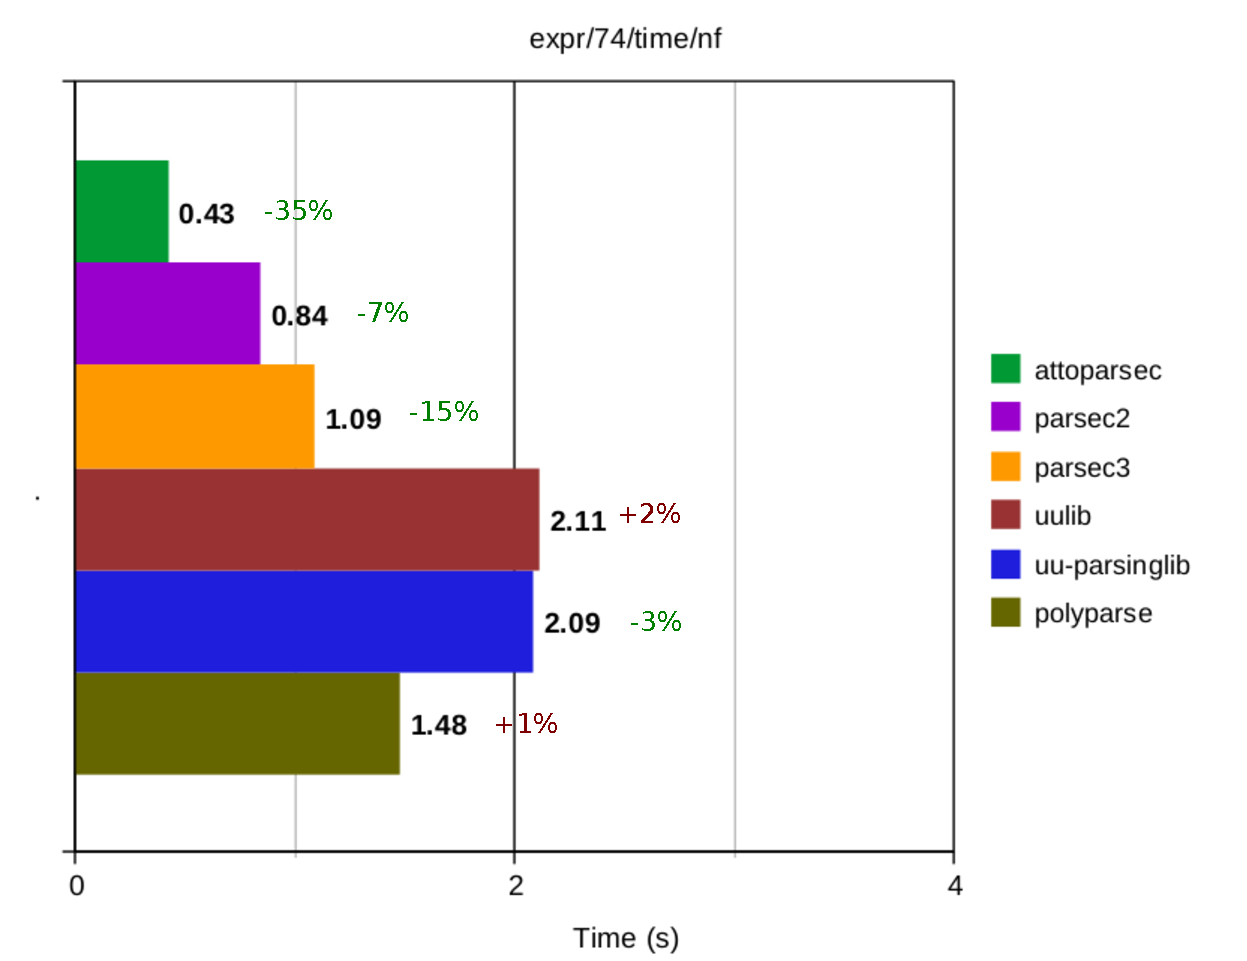
\includegraphics[scale=0.5]{presentation/expr-74-time-nf_.pdf}
\end{frame}

\begin{frame}{EXPR - Space}
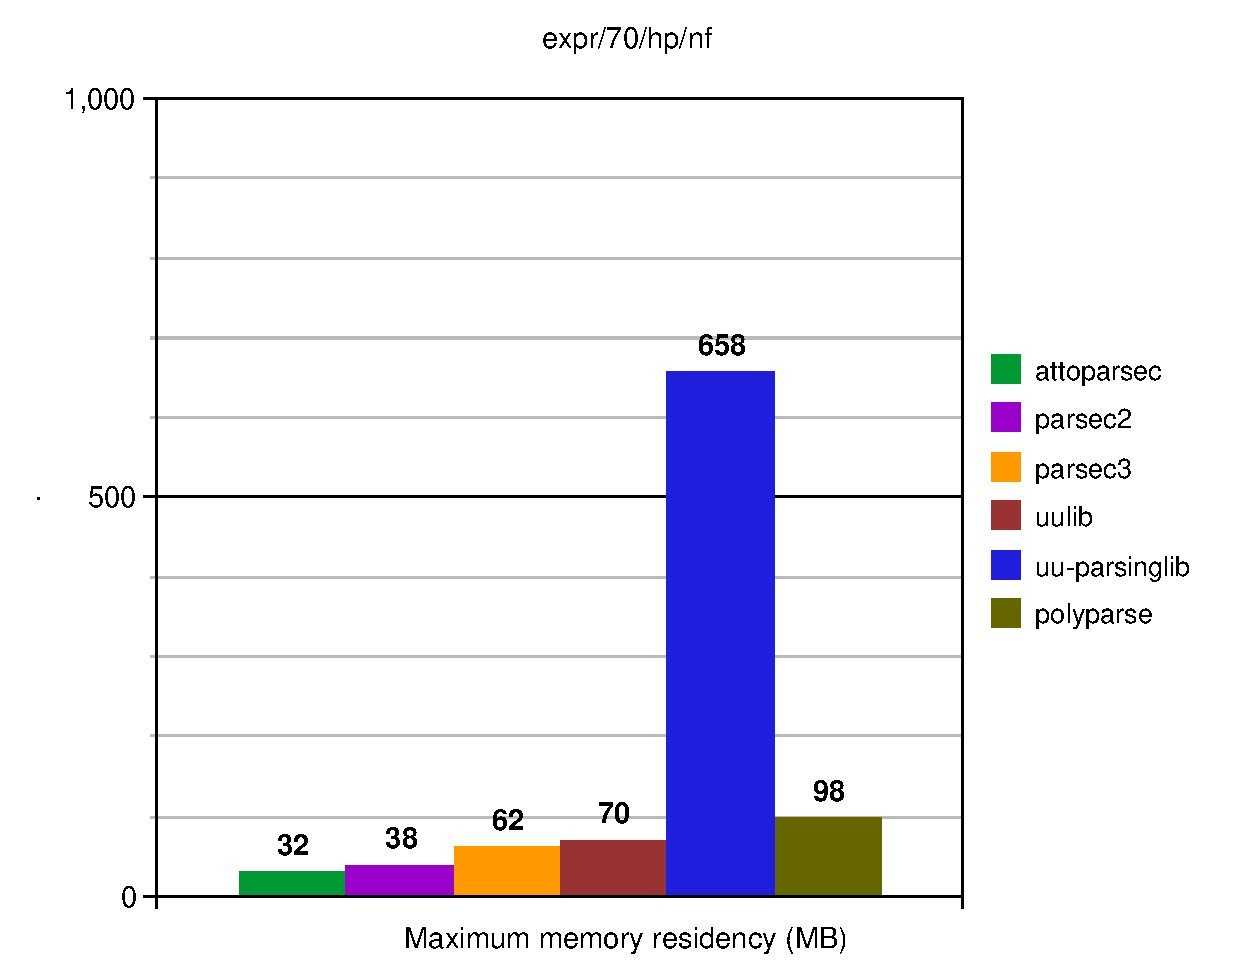
\includegraphics[scale=0.5]{presentation/expr-70-hp-nf.pdf}
\end{frame}

\begin{frame}[fragile]{URL - Example}
\begin{itemize}
\item URL query string
\item Datasets generated from previous CSV
\end{itemize}
\begin{verbatim}
Aachen&Aalborg=aah&Aalesund=aahed&Aalst=aahing&Aalto=aahs
&Aarau=aal&Aargau&Aarhus&Aaron=aals&Aarons+rod=aardvark
&Aaronic=aardwolf&Ab=aargh&Abadan&Abaddon=aarrghh&Abba=
aas&Abbasid=aasvogel&Abbevillian=aba&Abbey+Theatre=abaca&
\end{verbatim}
\end{frame}

\begin{frame}{URL - Time}
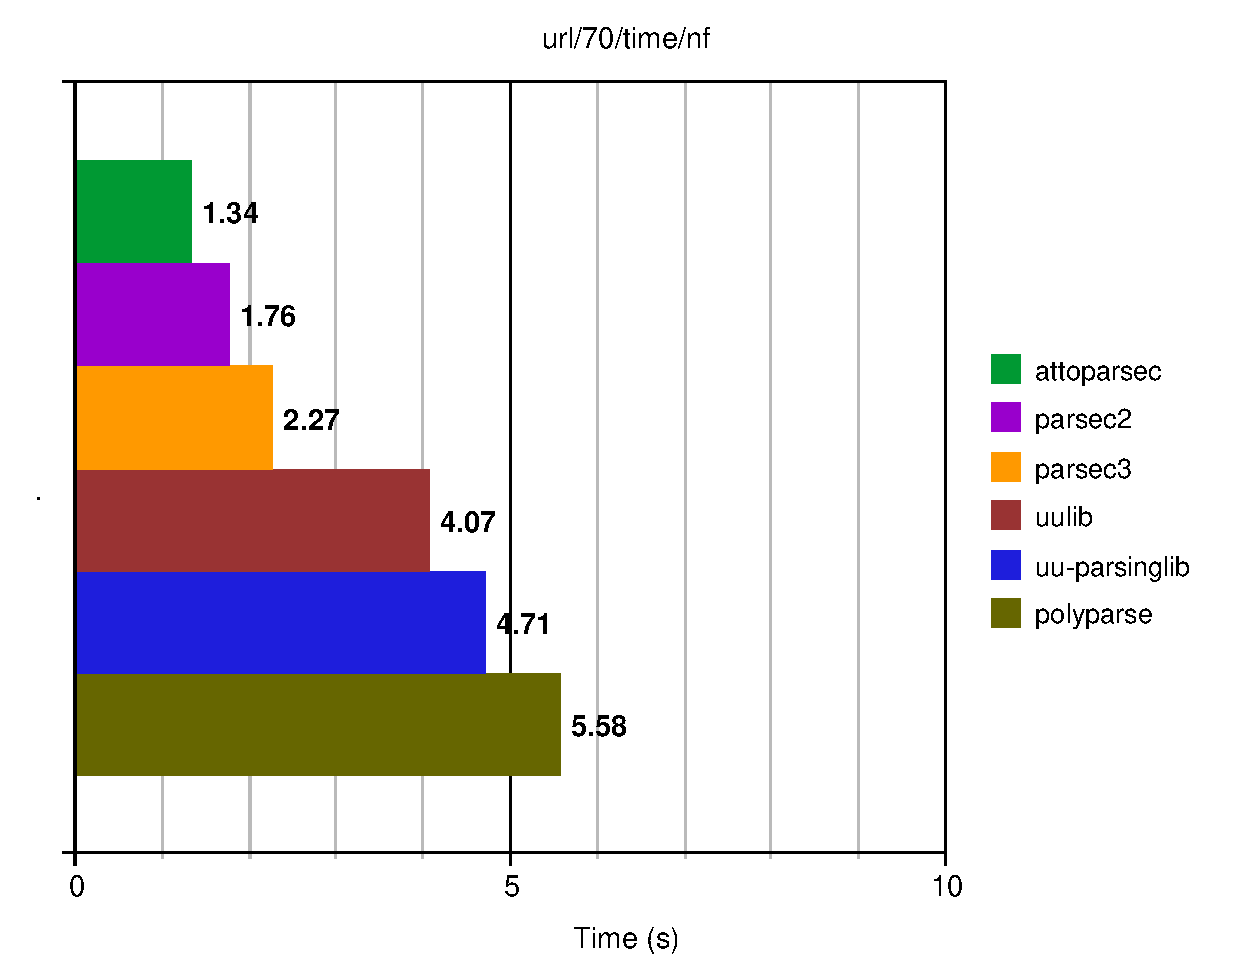
\includegraphics[scale=0.5]{presentation/url-70-time-nf.pdf}
\end{frame}

\begin{frame}{URL - Time - 74}
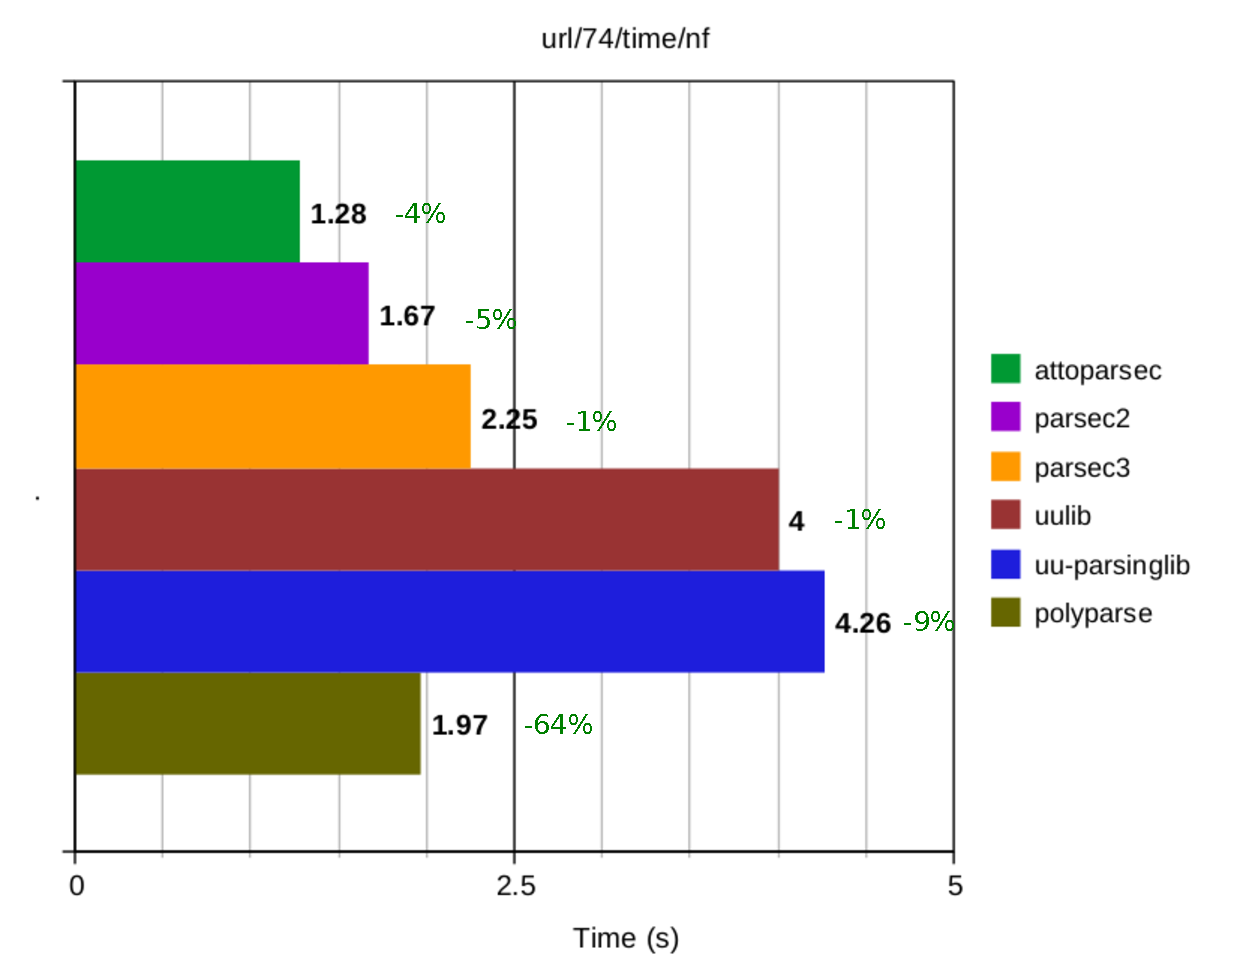
\includegraphics[scale=0.5]{presentation/url-74-time-nf_.pdf}
\end{frame}

\begin{frame}{URL - Space}
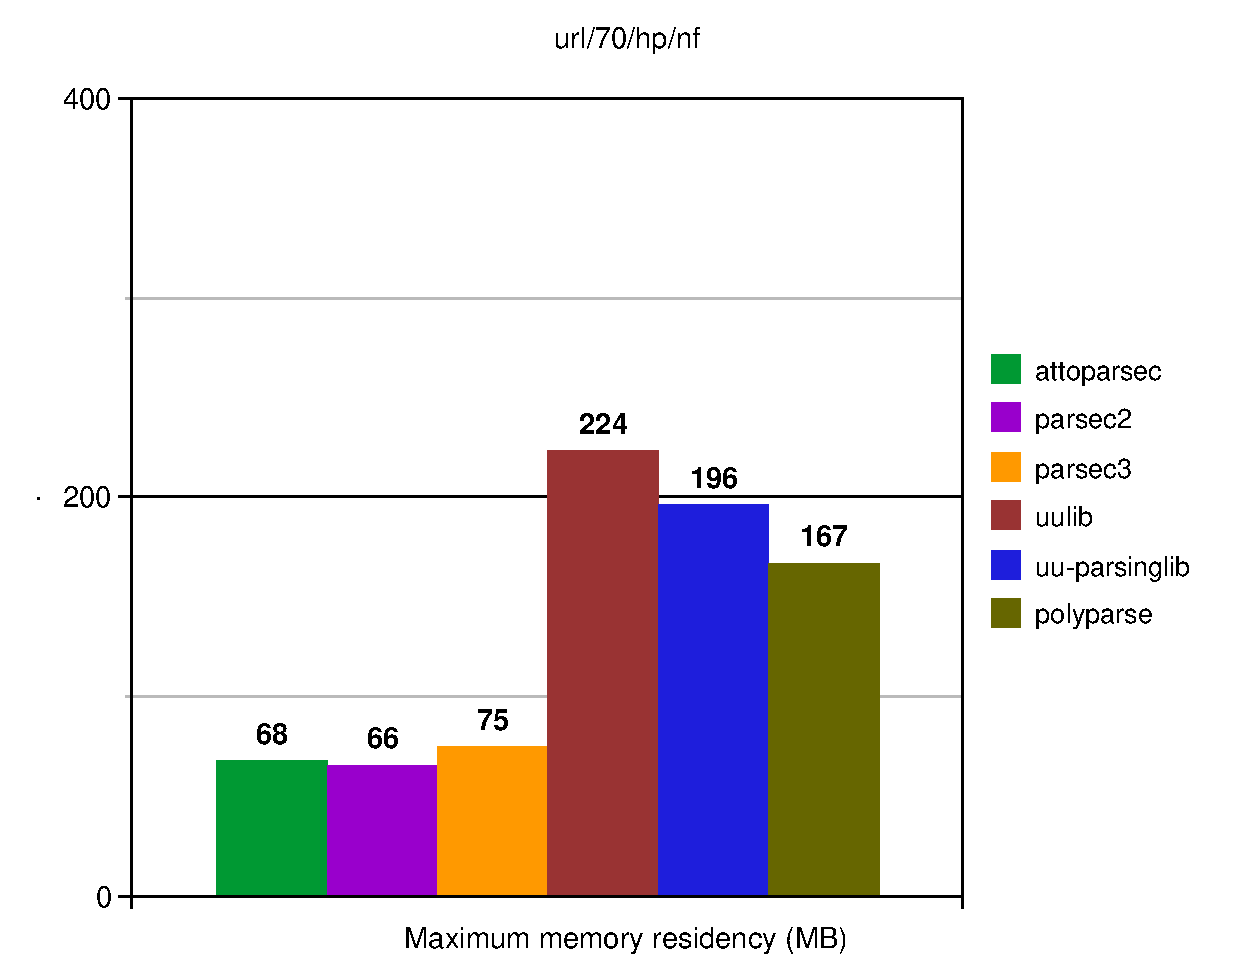
\includegraphics[scale=0.5]{presentation/url-70-hp-nf.pdf}
\end{frame}

\begin{frame}[fragile]{HTTP - Example}
\begin{itemize}
\item HTTP GET and POST requests
\item Datasets generated from previous CSV
\end{itemize}
\begin{verbatim}
POST http://www.w3.org/#sec3.6.1 HTTP/1.1
Aachen: aa
Aalborg: aah
Aalesund: aahed
Aalst: aahing
Aalto: aahs
Aarau: aal
Aargau: aalii
\end{verbatim}
\end{frame}

\begin{frame}{HTTP - Time}
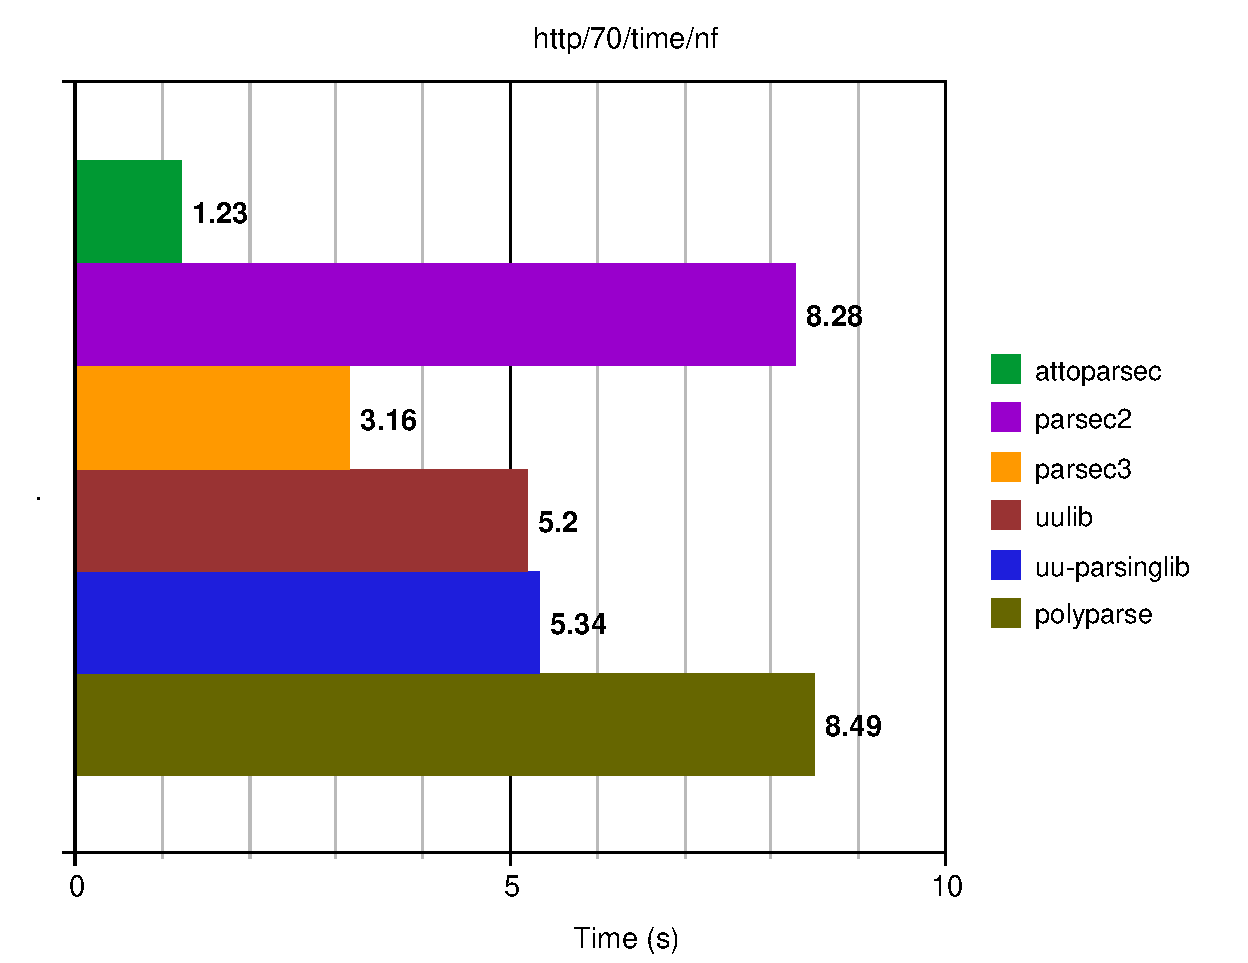
\includegraphics[scale=0.5]{presentation/http-70-time-nf.pdf}
\end{frame}

\begin{frame}{HTTP - Time - 74}
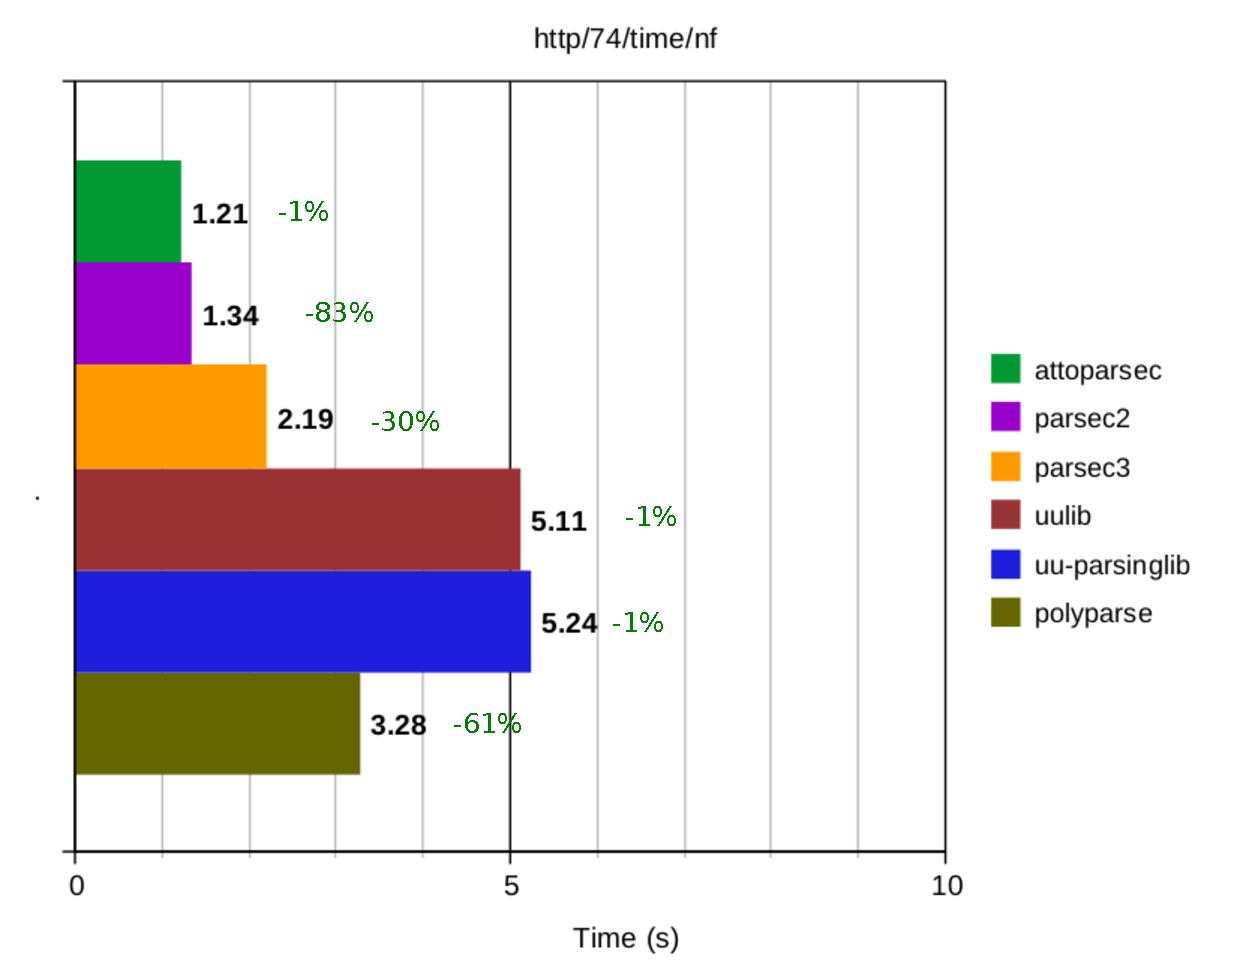
\includegraphics[scale=0.5]{presentation/http-74-time-nf_.pdf}
\end{frame}

\begin{frame}{HTTP - Space}
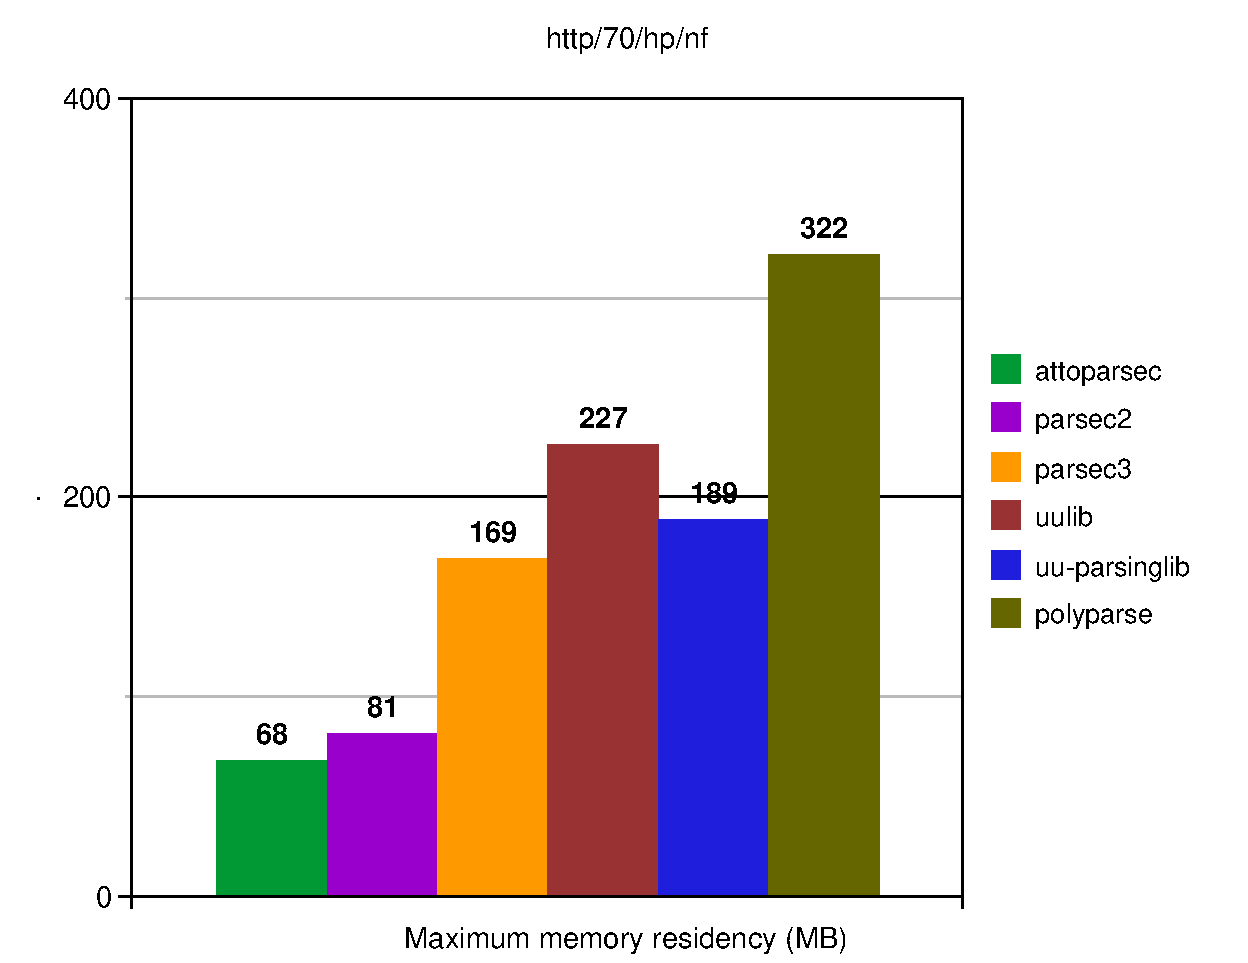
\includegraphics[scale=0.5]{presentation/http-70-hp-nf.pdf}
\end{frame}

\begin{frame}[fragile]{JSON - Example}
\begin{itemize}
\item Javascript Object Notation
\item Datasets collected from GitHub
\end{itemize}

\begin{verbatim}
{"030200b_.mid": [[{"timesig": null, "keysig": 2, "st": 0, 
"pitch": 50, "dur": 12.0, "fermata": 0}, {"timesig": null, 
"keysig": 2, "st": 12.0, "pitch": 49, "dur": 2.0, 
"fermata": 0}]]}
\end{verbatim}
\end{frame}

\begin{frame}{JSON - Time}
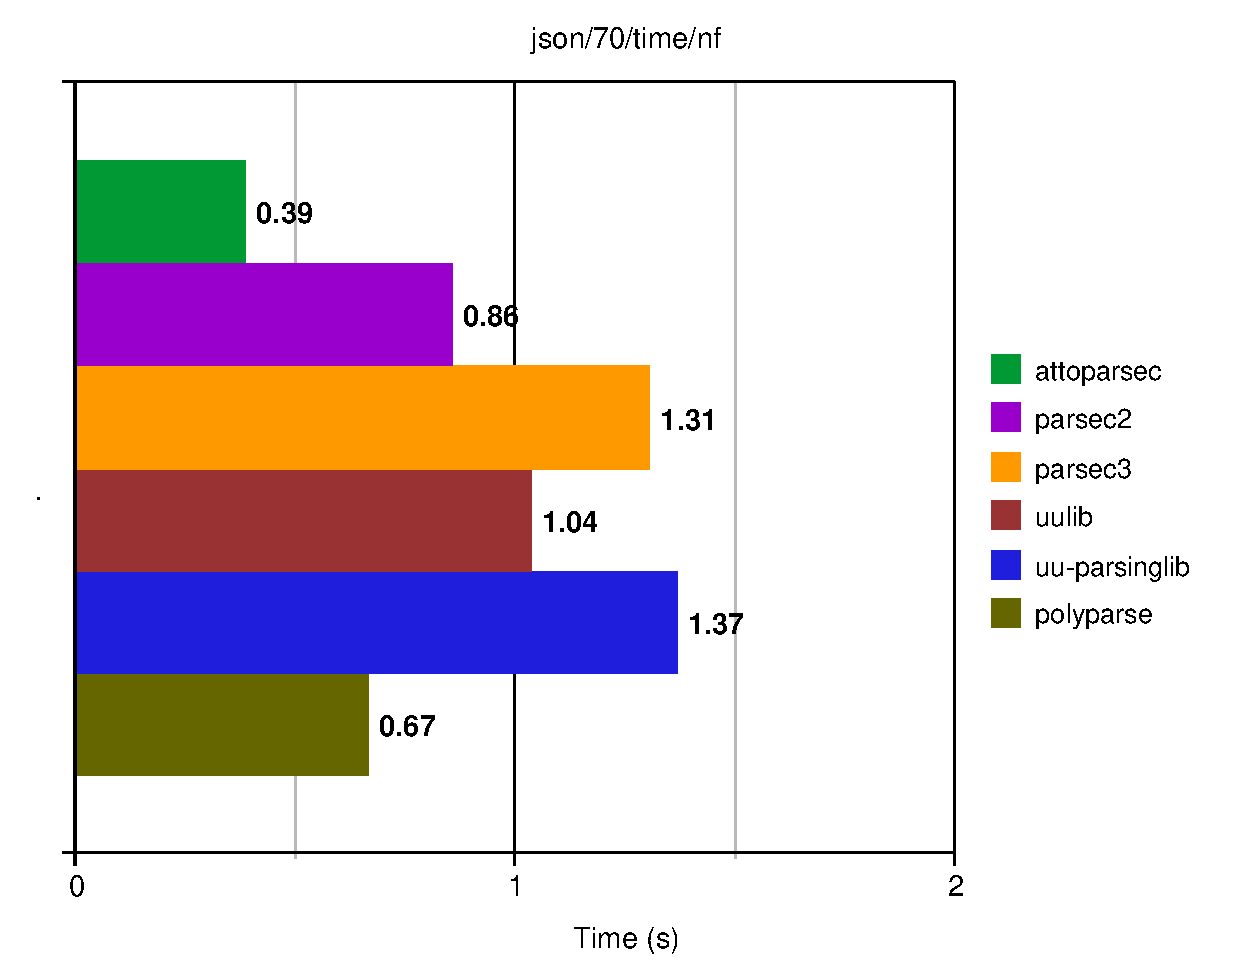
\includegraphics[scale=0.5]{presentation/json-70-time-nf.pdf}
\end{frame}

\begin{frame}{JSON - Time - 74}
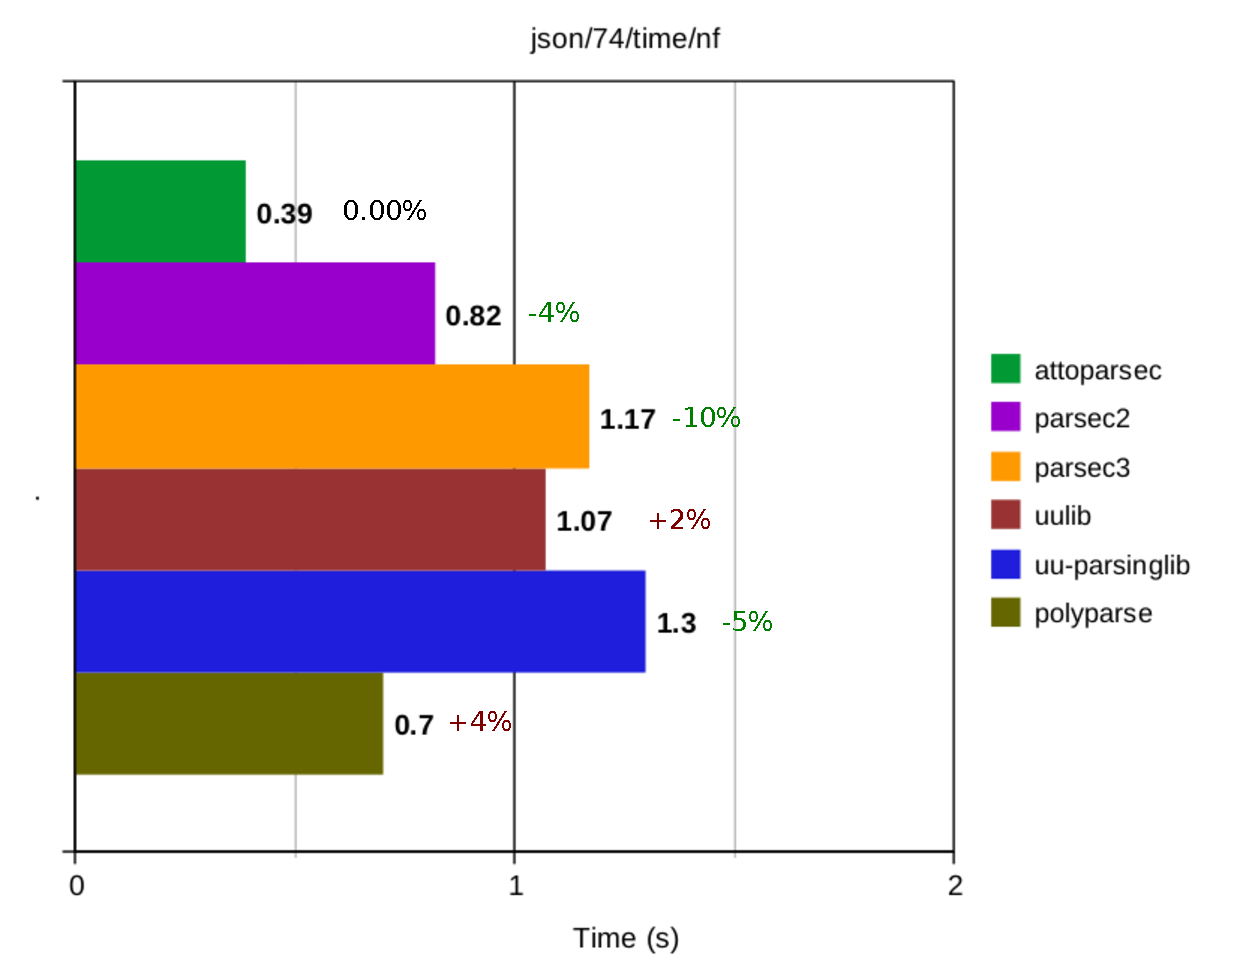
\includegraphics[scale=0.5]{presentation/json-74-time-nf_.pdf}
\end{frame}

\begin{frame}{JSON - Space}
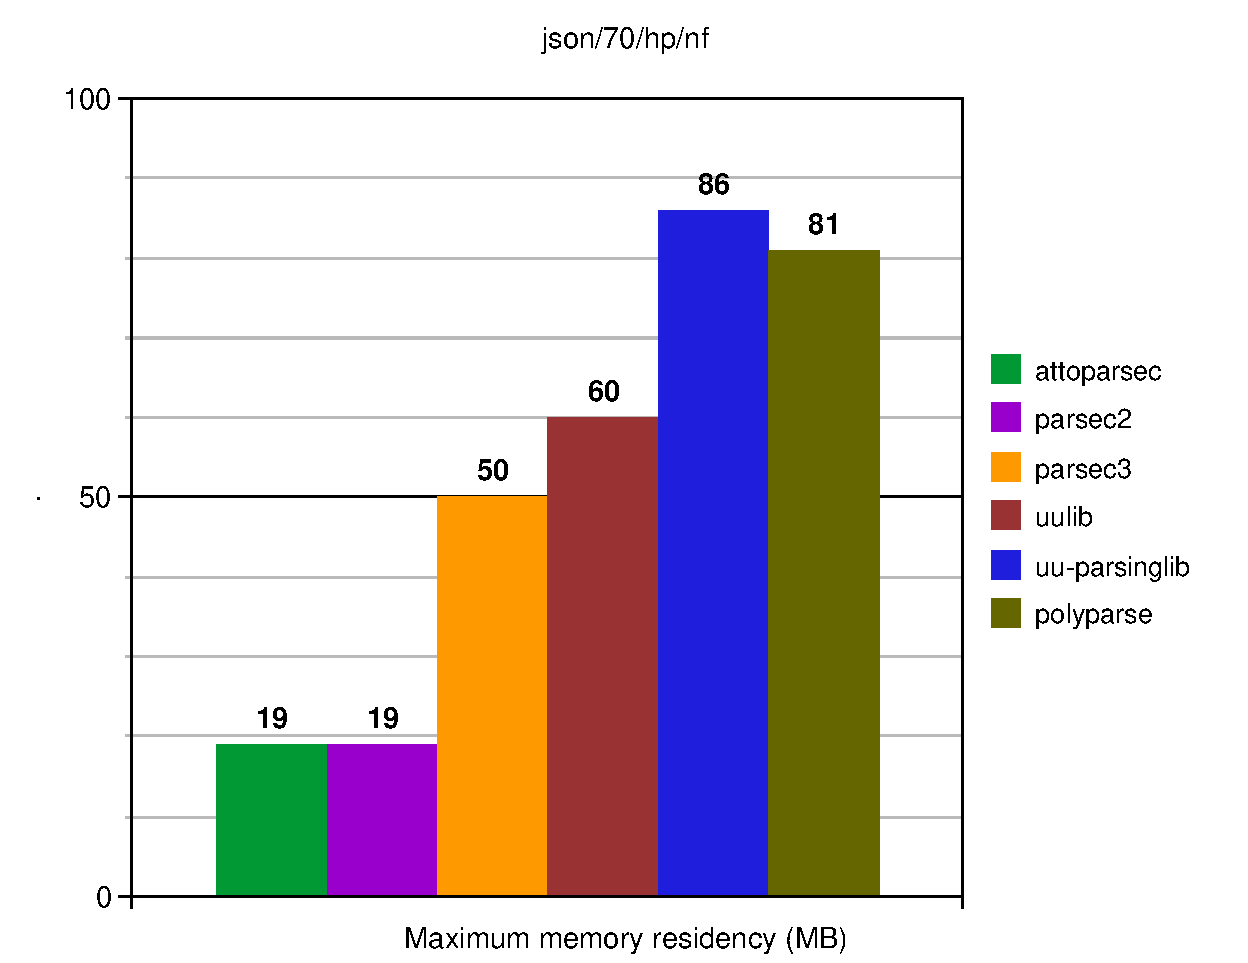
\includegraphics[scale=0.5]{presentation/json-70-hp-nf.pdf}
\end{frame}

\begin{frame}[fragile]{CSS - Example}
\begin{itemize}
\item Cascading Style Sheets
\item Datasets collected from GitHub
\end{itemize}
\begin{verbatim}
body{
  background-color: #222;
  color: white;
  font-family: "Bitstream Vera Sans",sans-serif;
  margin: 0;
  padding: 0;
}
#container{
  margin: 0 10%;
  background-color: #161616;
  padding: 16px;
}
\end{verbatim}
\end{frame}

\begin{frame}{CSS - Time}
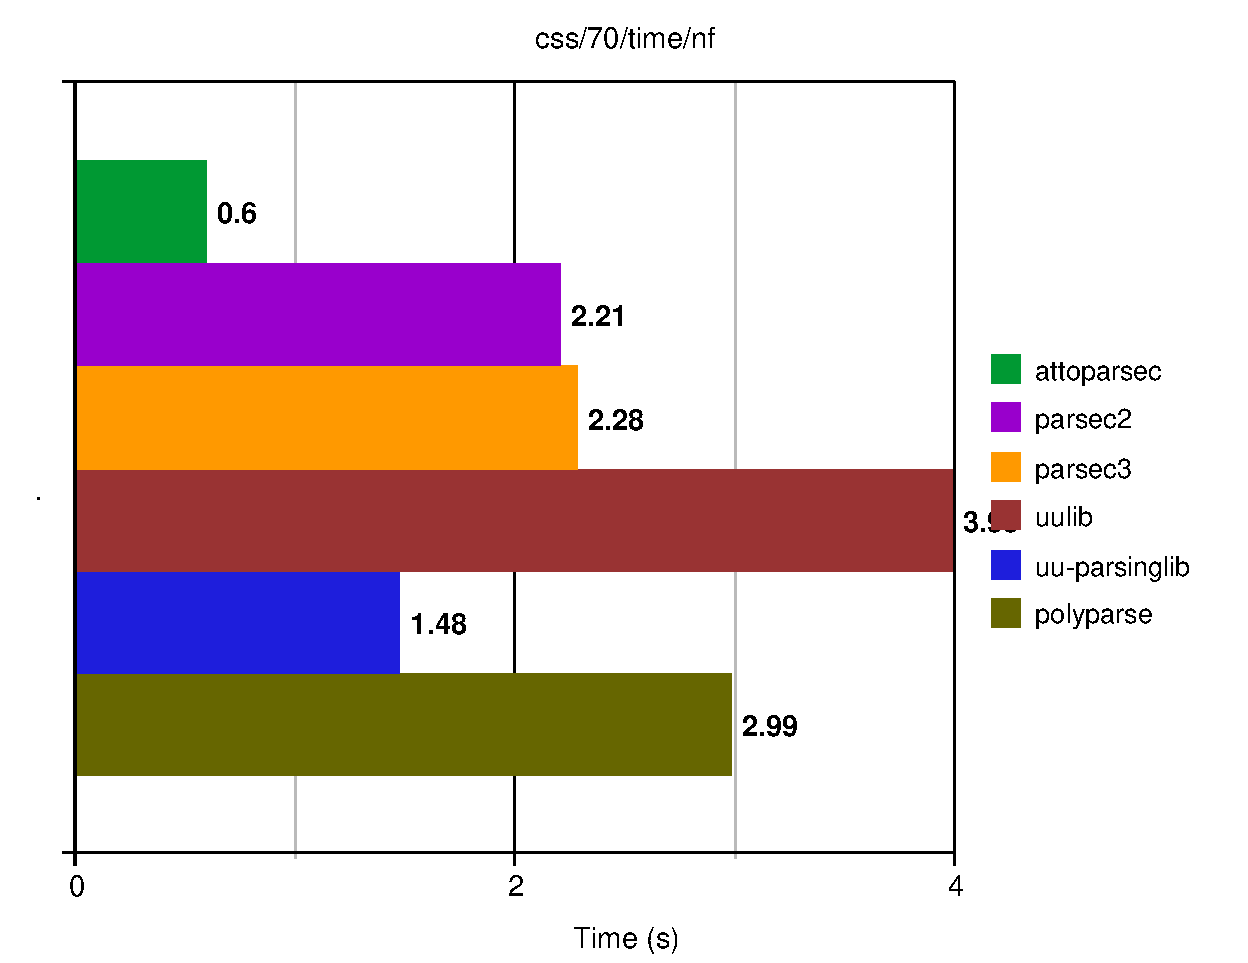
\includegraphics[scale=0.5]{presentation/css-70-time-nf.pdf}
\end{frame}

\begin{frame}{CSS - Time - 74}
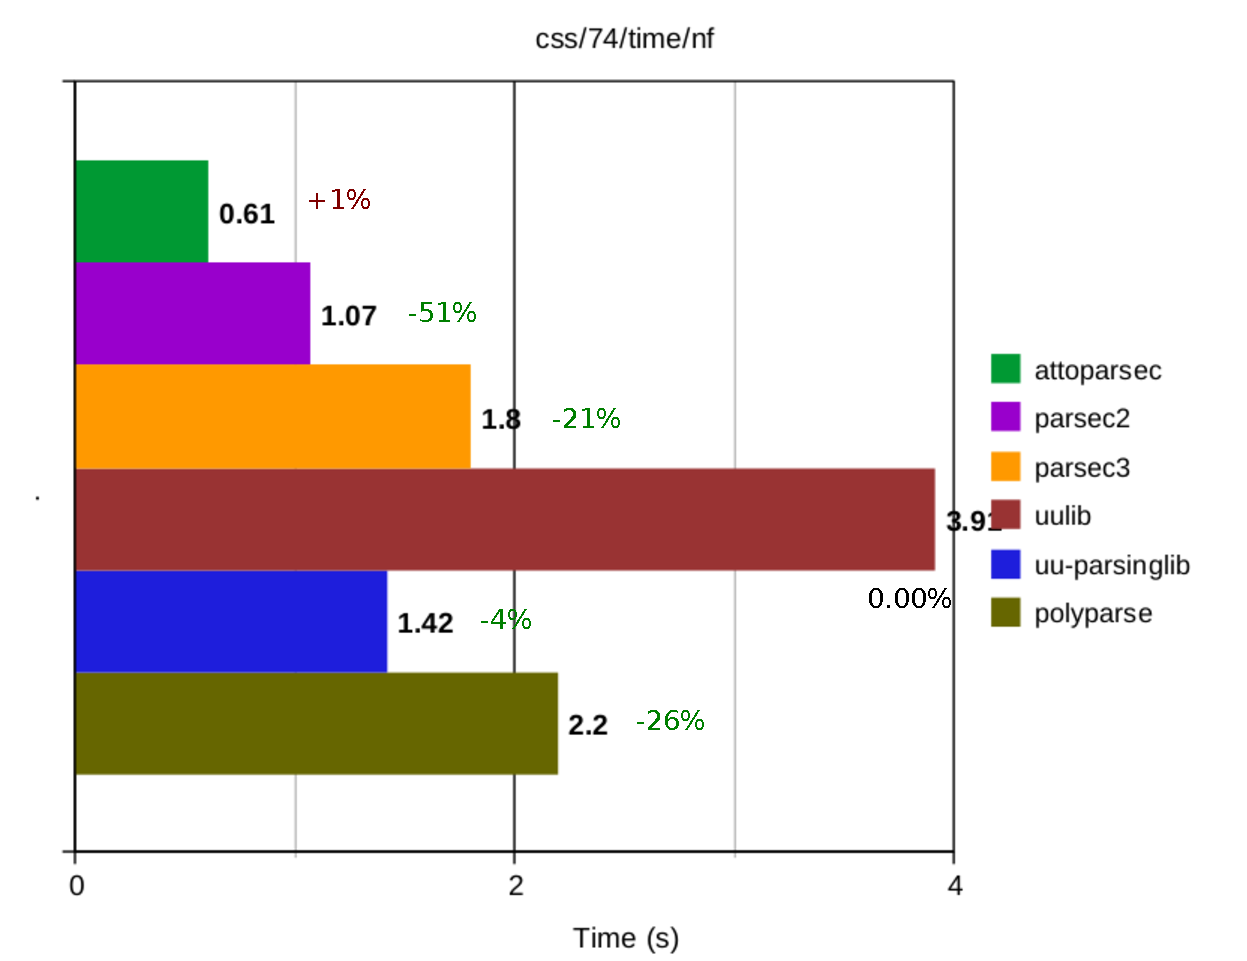
\includegraphics[scale=0.5]{presentation/css-74-time-nf_.pdf}
\end{frame}

\begin{frame}{CSS - Space}
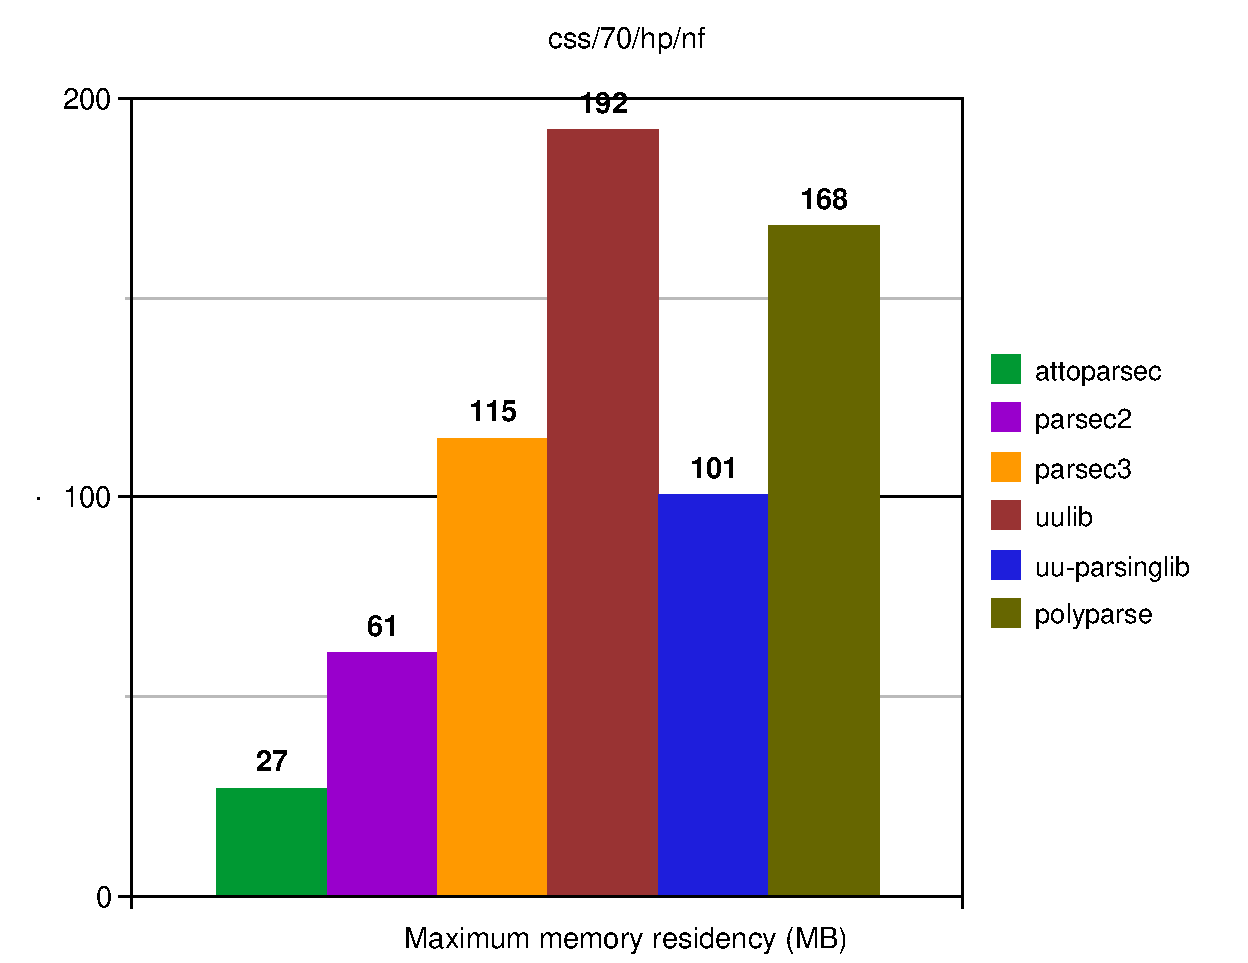
\includegraphics[scale=0.5]{presentation/css-70-hp-nf.pdf}
\end{frame}

\begin{frame}{UU-parsinglib Online - Space}
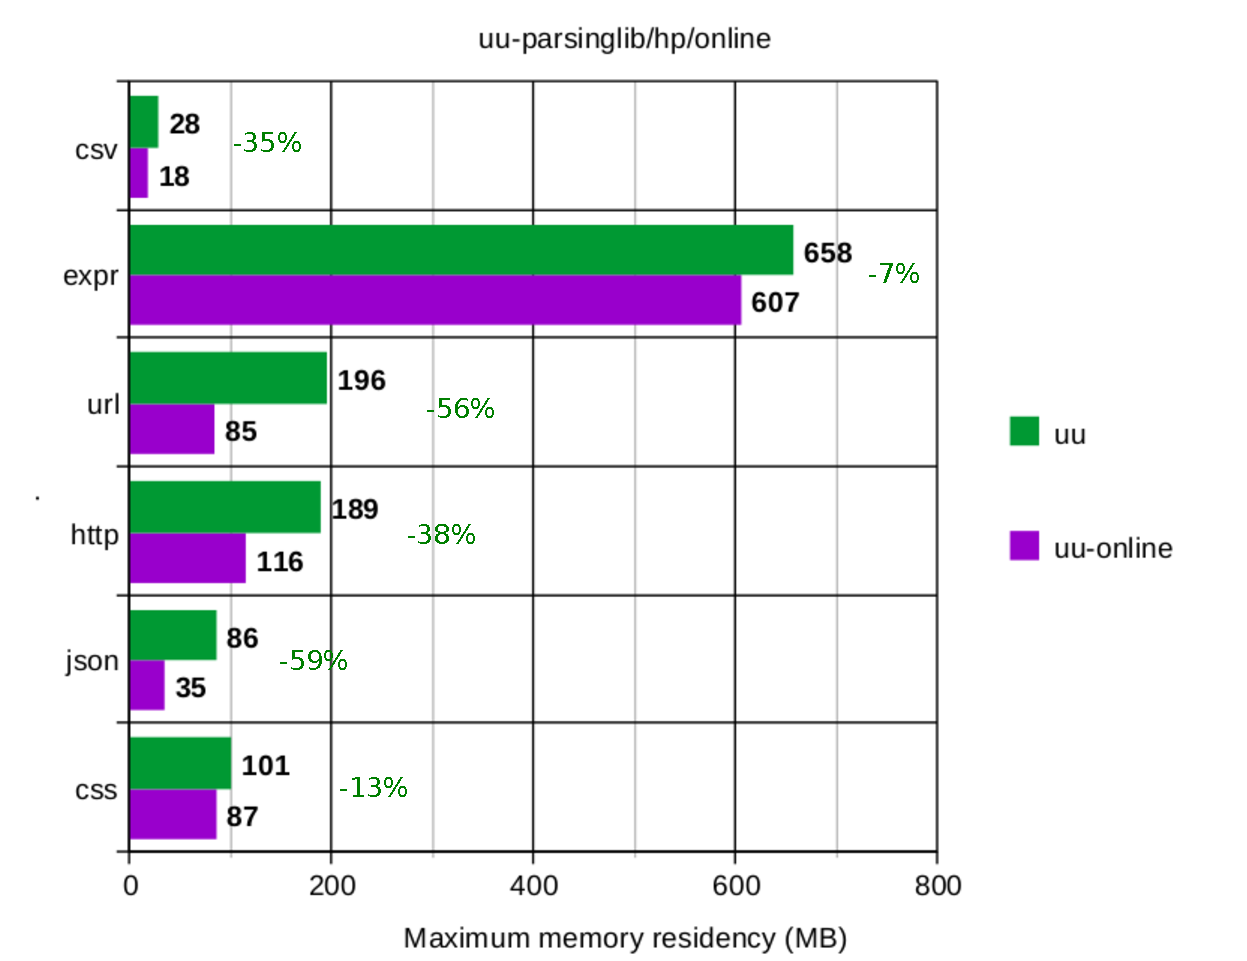
\includegraphics[scale=0.5]{presentation/uu-parsinglib-hp-online_.pdf}
\end{frame}

\begin{frame}{UU-parsinglib Online - Time}
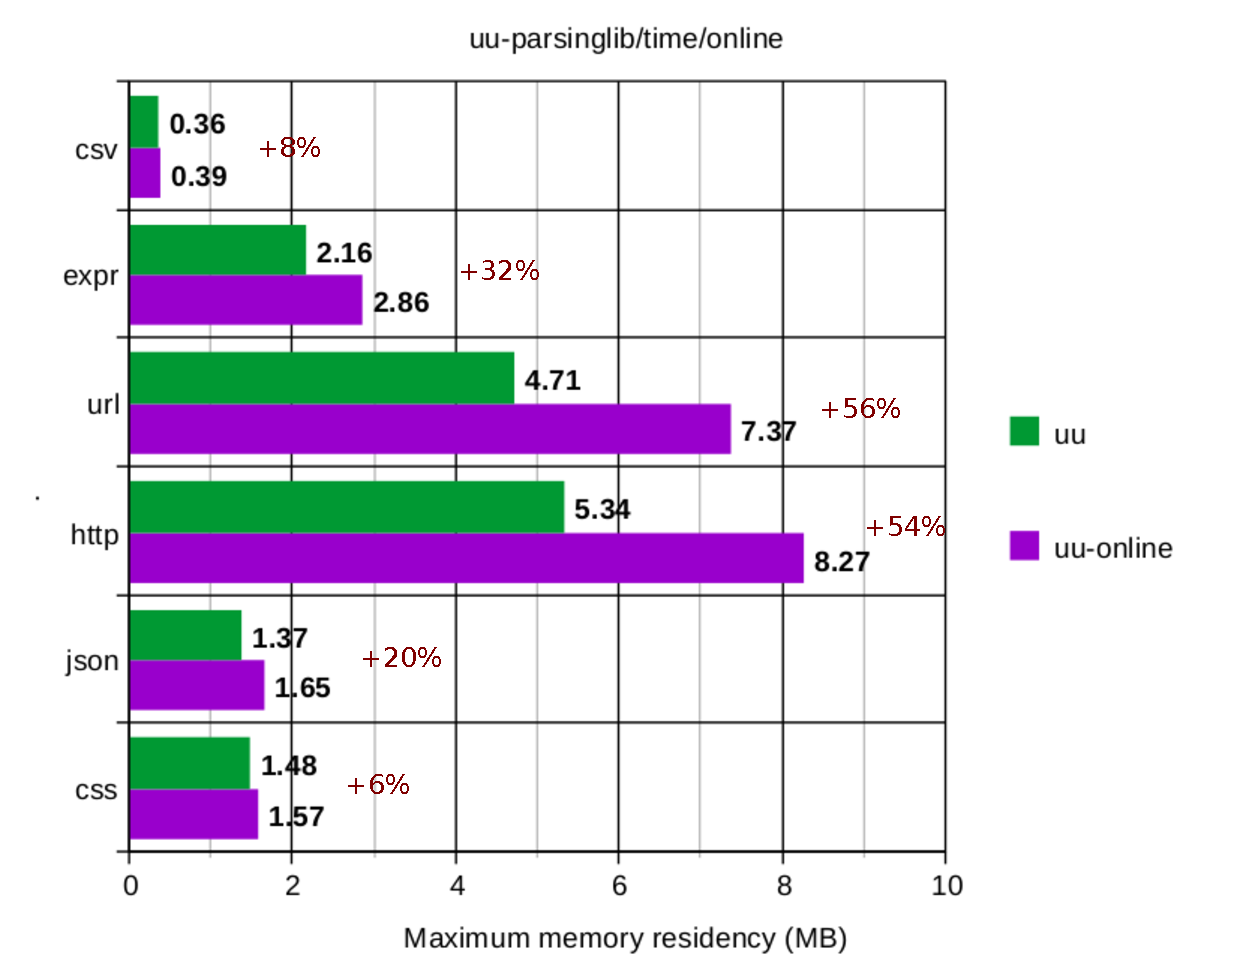
\includegraphics[scale=0.5]{presentation/uu-parsinglib-time-online_.pdf}
\end{frame}

\begin{frame}{UU-parsinglib Data.Text - Space}
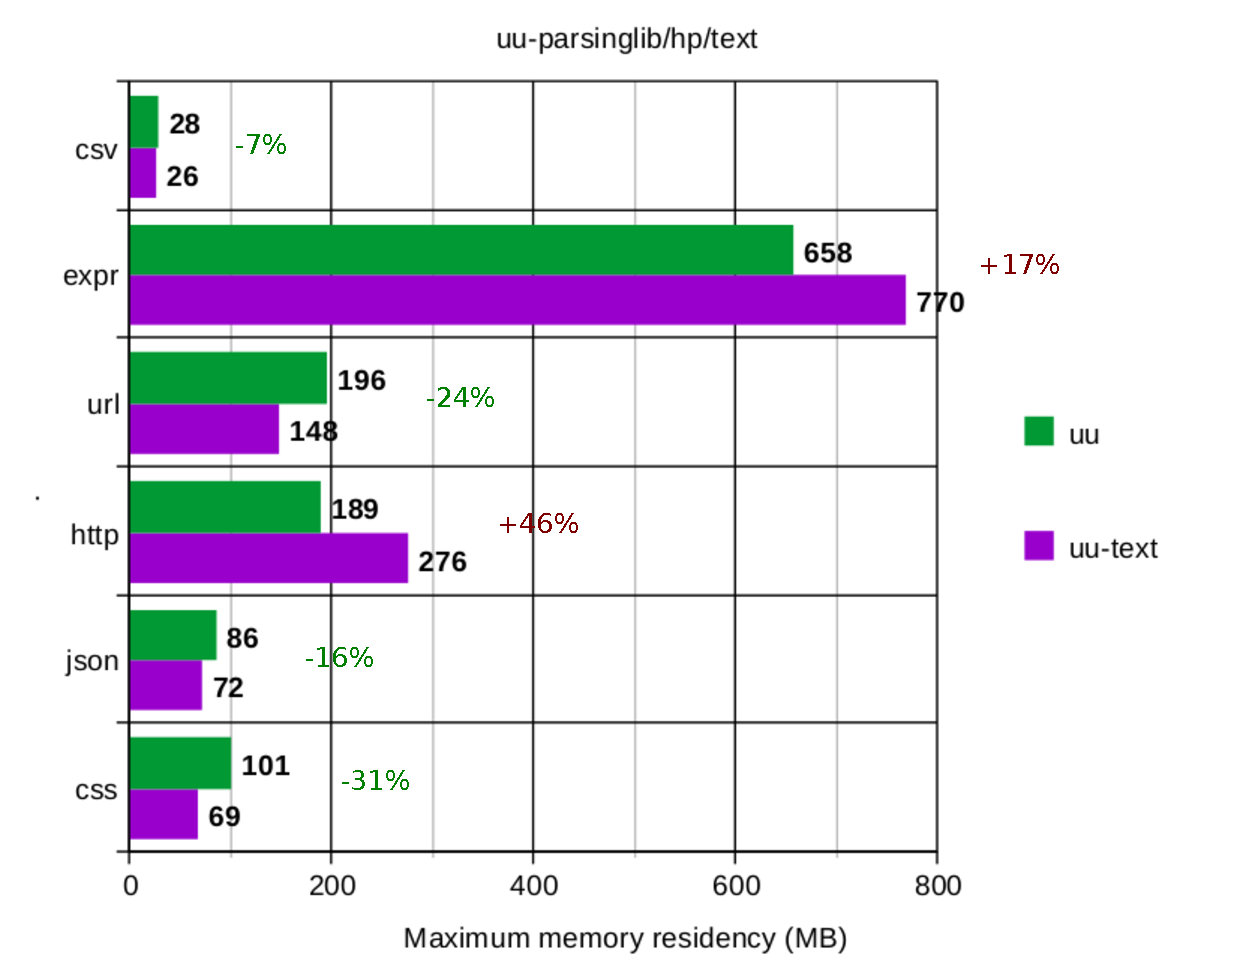
\includegraphics[scale=0.5]{presentation/uu-parsinglib-hp-text_.pdf}
\end{frame}


\begin{frame}{Overall results}
\begin{itemize}
\item GHC 7.4 brings a 15\%  performance increase
\item WHNF 17\% faster than NF on the test
\item WHNF uses 16\% less memory than NF
\end{itemize}
\end{frame}

\section{Outro}

\begin{frame}{How the results were produced}
\begin{itemize}
\item My slow laptop
\item Archlinux x86\_64
\item GHC 7.0.3 and GHC 7.4.1
\item Latest versions of parsing libraries
\item Criterion
\item Virthualenv
\item Custom profiling scripts
\end{itemize}
\end{frame}

\begin{frame}{Conclusion \& Impressions}
\begin{itemize}
\item attoparsec is the winner on almost all benchmarks
\item parsec2 is faster than parsec 3 on all benchmarks (GHC 7.4)
\item uu-parsinglib is the best abstracted away
\item uu-parsinglib online feature is benifitial albeit slower
\item was expecting a larger boost with Data.Text 
\item WHNF is slightly faster than NF for all contenstants, but does not affect the results ordering
\end{itemize}

\end{frame}

\begin{frame}{Suggestions \& Future Work}
\begin{itemize}
\item Revise the parsers
\item Try to squeeze even the last drop of speed
\item Add more example cases
\item It would be nice if there was a similar tool to Criterion
but for profiling comparisons
\end{itemize}
\end{frame}

\end{document}

